\section{Esposizione
dell\textquotesingle Architettura}\label{esposizione-dellarchitettura}

La topologia e\textquotesingle{} suddivisa logicamente in due reti:

\begin{itemize}
\tightlist
\item
  \textbf{Una rete di produzione per ogni team}, dove la rete
  \(\text{production-}k\) identifica gli oggetti di rete usati per
  collegare i container vulnerabili alla rete per il team \(k\)
\item
  \textbf{Al piu\textquotesingle{} una rete di verifica per ogni team},
  dove la rete \(\text{verify-}k\) identifica gli oggetti di rete ed i
  container duplicati utilizzati per la verifica richiesta dal
  \(\text{team-}k\)
\end{itemize}

Dunque schema di indirizzamento prevede una netta separazione tra lo
spazio di gioco del team \(k\), la rete WireGuard e la rete di Incus:

\begin{itemize}
\tightlist
\item
  \passthrough{\lstinline!10.k.0.0/24!}: sottorete WireGuard per i
  membri del team \(k\).
\item
  \passthrough{\lstinline!10.k.1.0/24!}: sottorete LAN per i container
  di produzione e per i cloni di verifica.
\item
  \passthrough{\lstinline!172.16.0.0/24!}: sottorete gestita da
  \(\text{incusbr0}\) per fornire la connettività esterna e le reti OVN
  tramite NAT.
\end{itemize}

\subsection{\texorpdfstring{rete
\(\text{production-}k\)}{rete \textbackslash text\{production-\}k}}\label{rete-textproduction-k}

La rete \(\text{production-}k\) e\textquotesingle{} fatta cosi,
contiene:

\begin{itemize}
\tightlist
\item
  \(\text{wg-}k\): dispositivo L3 gestito da WireGuard, fa da
  terminazione per il tunnel del team \(k\)-esimo. Ha come IP gateway:
  \passthrough{\lstinline!10.k.0.0/24!}
\item
  \(\text{br-team-}k\): dispositivo L2 gestito dal kernel Linux. Ha come
  IP gateway: \passthrough{\lstinline!10.k.1.0/24!}
\item
  \(\text{eth0}\): le interfacce di rete \(\text{eth0}\) dei container
  vengono collegate a \(\text{br-team-}k\).
\end{itemize}

\(\text{wg-}k\) serve per fronire ai membri del team \(k\)
l\textquotesingle endpoint per la connessione tramite VPN, in questo
modo i membri del team saranno connessi direttamente alla rete
\(\text{production-}k\). Ogni membro ha la sua configurazione WireGuard
associata al suo peer impostato sull\textquotesingle interfaccia
\(\text{wg-}k\). Aggiungere un peer all\textquotesingle interfaccia
WireGuard significa permettere ad un client con una certa chiave
pubblica di collegarsi con un certo indirizzo ip (\textbf{cryptokey
routing}), dunque ogni membro del team \passthrough{\lstinline!k!} ha il
suo indirizzo nella sottorete \passthrough{\lstinline!10.k.0.0/24!}.

L\textquotesingle interfaccia \(\text{br-team-}k\) permette di creare
una rete LAN per i container del team \(k\). Ogni interfaccia
\passthrough{\lstinline!eth0!} dei container istanziati dal team \(k\),
vengono "collegati" (tramite l\textquotesingle utilizzo di un profilo
Incus) a \(\text{br-team-}k\). La connessione tra bridge e container
viene gestita direttamente da Incus.

Questo collegamento avviene tramite l\textquotesingle utilizzo di una
\passthrough{\lstinline!veth pair!} (Virtual Ethernet) per container:
una estremita e\textquotesingle{} collegata a
\passthrough{\lstinline!br-team-k!}, l\textquotesingle altra
all\textquotesingle interffacia del container
\passthrough{\lstinline!eth0!}. Dunque all\textquotesingle interno del
kernel appesantiamo il carico nella gestione delle interfacce, infatti
avremmo oltre ad \passthrough{\lstinline!eth0!}, una coppia
\passthrough{\lstinline!veth!} per ogni container.

\begin{quote}
\passthrough{\lstinline!veth!}: E\textquotesingle{} utile per collegare
interfacce che risiedono per esempio su differenti Network Namespace
(ossia il modo in cui sono implementati i container). Utilizzano poca
CPU e poca memoria, dato che l\textquotesingle implementazione risiede
direttamente nel kernel. Dunque per centinaia di
\passthrough{\lstinline!veth!} non si ha un degrado evidente delle
prestazioni. \footnote{\label{fn:ref_15}\url{https://dev.to/godofgeeks/virtual-ethernet-devices-veth-ofd}}
\end{quote}

Tramite regole di routing, il traffico dell\textquotesingle interfaccia
\(\text{wg-}k\) viene instradato verso \(\text{br-team-}k\) e viceversa.
Il routing viene applicato aggiungendo al sistema, dentro al set
\passthrough{\lstinline!team\_links!} la coppia di interfacce. Le regole
ed i comandi usati per implementare l\textquotesingle inoltro verranno
esposti piu avanti.


\begin{figure}[htbp]
  \centering
  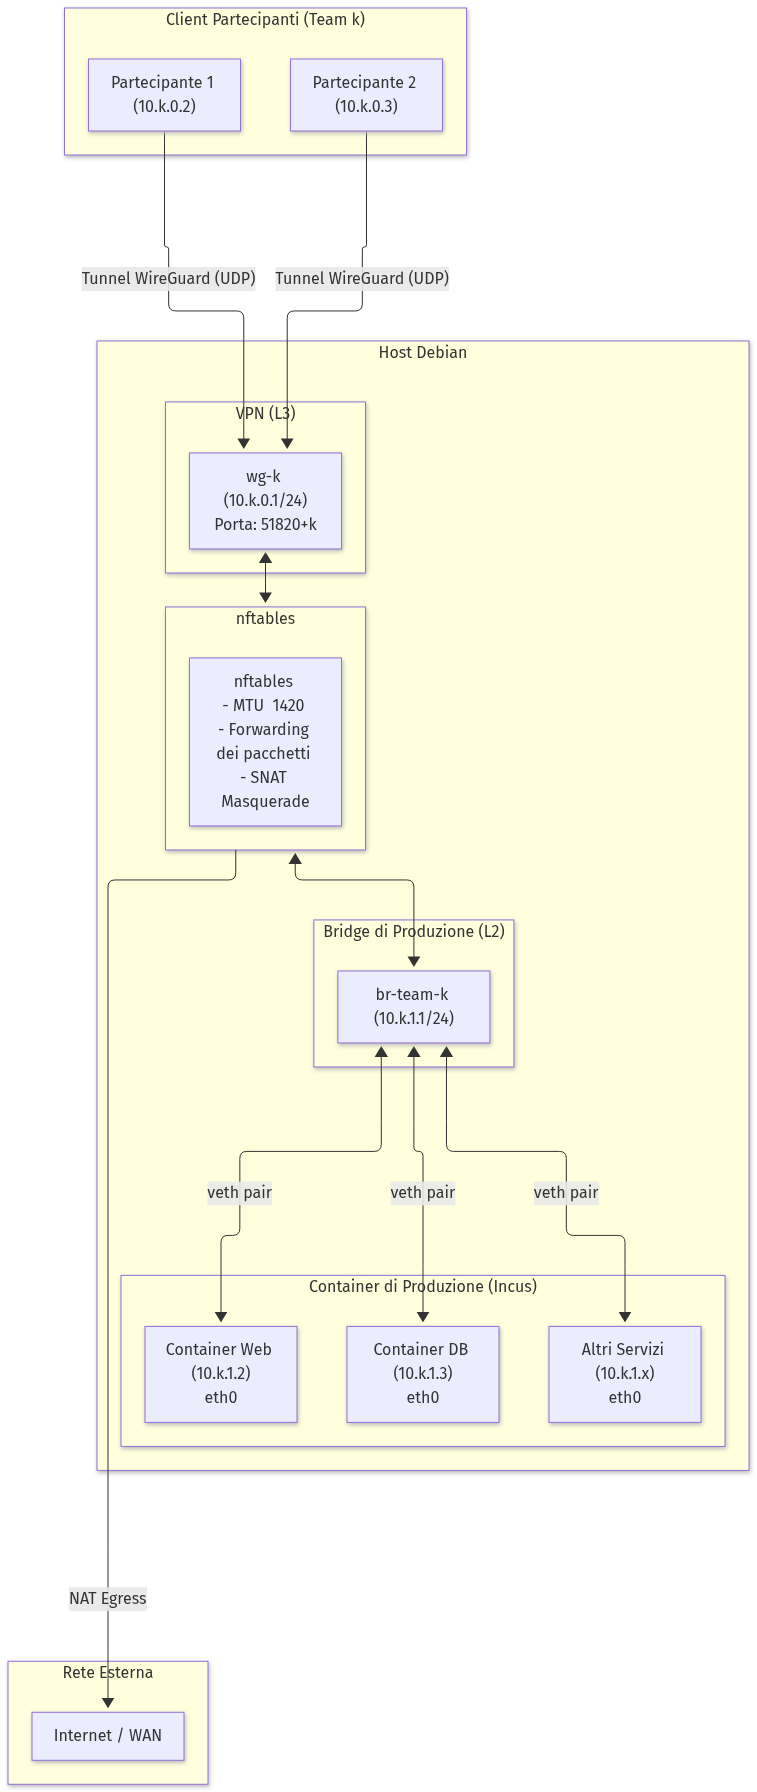
\includegraphics[width=0.92\linewidth,height=0.7\textheight,keepaspectratio]{src/images/mermaid_261_rete_production_k_fc40fab722.png}
  \caption{261 Rete Production K}
  \label{fig:mermaid_261_rete_production_k_fc40fab722}
\end{figure}


\begin{center}\rule{0.5\linewidth}{0.5pt}\end{center}

\subsection{\texorpdfstring{rete
\(\text{verify-}k\)}{rete \textbackslash text\{verify-\}k}}\label{rete-textverify-k}

La rete \(\text{verify-}k\) e\textquotesingle{} fatta cosi, contiene:

\begin{itemize}
\tightlist
\item
  \(\text{verify-ovn-}k\): rete virtuale logica gestita via SDN tramite
  OVN e orchestrata da Incus \footnote{\label{fn:ref_16}Documentazione ufficiale Incus,
    OVN network driver:
    \url{https://linuxcontainers.org/incus/docs/main/reference/network_ovn/}}.
  Non costituisce una singola interfaccia di rete convenzionale del
  kernel, ma una topologia virtuale isolata composta da uno switch e un
  router con gateway: \passthrough{\lstinline!10.k.1.1/24!}.
\item
  \(\text{incusbr0}\): bridge di rete di Incus sull\textquotesingle host
  con gateway \passthrough{\lstinline!172.16.0.1/24!}. Svolge il ruolo
  di interfaccia per l\textquotesingle instradamento verso
  l\textquotesingle esterno della rete OVN.
\item
  \(\text{eth0}\): sono le interfacce di rete dei container clonati
  (\passthrough{\lstinline!10.k.1.x!}) che vengono collegate a
  \(\text{verify-ovn-}k\).
\end{itemize}

\begin{quote}
Incus e\textquotesingle{} in grado di gestire da solo il collegamento
tra \(\text{incusbr0}\) ed \(\text{verify-ovn-}k\). Questo semplifica di
molto la gestione delle interfacce di verifica per BlueAgent.
\end{quote}

Le interfacce dei container e la rete \(\text{verify-ovn-}k\) sono
gestite dalla SDN (\emph{Software Defined Network}).
\(\text{verify-ovn-}k\) e\textquotesingle{} implementata da:

\begin{enumerate}
\def\labelenumi{\arabic{enumi}.}
\tightlist
\item
  un \textbf{Logical Switch} (denominato internamente da Incus nel DB di
  OVN come \passthrough{\lstinline!incus-net<ID>-ls-int!} \footref{fn:ref_16}):
  rappresenta la LAN su cui si agganciano le interfacce virtuali dei
  container di verifica.
\item
  un \textbf{Logical Router} (denominato
  \passthrough{\lstinline!incus-net<ID>-lr!} \footref{fn:ref_16}):
  agisce come gateway (\passthrough{\lstinline!10.k.1.1/24!}),
  permettendo ai container clonati di preservare
  l\textquotesingle identica configurazione IP rispetto alla produzione.
\end{enumerate}

\begin{quote}
\textbf{Tunneling Geneve e considerazioni sull\textquotesingle MTU:} OVN
impiega il protocollo di tunneling \textbf{Geneve} (\emph{Generic
Network Virtualization Encapsulation}) \footnote{\label{fn:ref_17}Documentazione
  architetturale OVN e Geneve:
  \url{https://docs.ovn.org/en/latest/topics/geneve.html}} per
realizzare la rete overlay, incapsulando i frame L2
all\textquotesingle interno di pacchetti UDP. Il tunnel Geneve opera
interamente confinato all\textquotesingle interno
dell\textquotesingle host, isola il traffico di verifica impedendo che
transiti sulle interfacce di rete visibili ai partecipanti.
\end{quote}

L\textquotesingle incapsulamento Geneve introduce tuttavia un overhead
di intestazione di 58 byte, riducendo l\textquotesingle MTU effettiva
della rete di verifica a \(1442\) byte (rispetto ai 1500 byte standard).
In combinazione con il tunnel WireGuard (avente MTU \(1420\)), abbiamo
una riduzione complessiva del \emph{Path MTU}. Se pacchetti di
dimensione eccedente hanno il flag \emph{Don\textquotesingle t Fragment}
(DF) abilitato, rischiano di essere scartati generando un fenomeno di
\emph{Path MTU Blackhole}. Questo problema viene risolto forzando il
\emph{clamping} del MSS per il traffico TCP via
\passthrough{\lstinline!nftables!} \footnote{\label{fn:ref_18}Documentazione Netfilter,
  TCP MSS Clamping:
  \url{https://wiki.nftables.org/wiki-nftables/index.php/Forwarding_traffic}},
mentre il traffico UDP deve rimanere entro i limiti imposti
dall\textquotesingle MTU minima della catena.

Questo approccio \emph{garantisce l\textquotesingle assenza di conflitti
di routing} grazie a una netta separazione tra \textbf{spazio utente} e
\textbf{spazio kernel} \footnote{\label{fn:ref_19}Documentazione Open vSwitch,
  architettura Datapath Kernel vs Userspace:
  \url{https://docs.openvswitch.org/en/latest/intro/what-is-ovs/}}:

\begin{itemize}
\tightlist
\item
  \textbf{Spazio Utente (Control Plane):} i demoni di controllo di OVN
  (\passthrough{\lstinline!ovn-controller!},
  \passthrough{\lstinline!ovn-northd!}) e di Open vSwitch
  (\passthrough{\lstinline!ovs-vswitchd!}) elaborano la topologia logica
  e la traducono in flussi OpenFlow. Il router OVN esiste puramente a
  questo livello logico fino ad ora esiste solo logicamente.
\item
  \textbf{Spazio Kernel (Data Plane):} l\textquotesingle effettivo
  inoltro dei frame avviene ad alte prestazioni tramite il modulo kernel
  di Open vSwitch. Il kernel gestisce una tabella di flussi in cache
  (\emph{datapath flow cache}), instradando e modificando i pacchetti
  senza passare dallo stack di rete IP standard
  dell\textquotesingle host.
\end{itemize}

Il collegamento tra i container e la rete OVN sfrutta sempre una coppia
\passthrough{\lstinline!veth pair!}: un\textquotesingle estremità
risiede all\textquotesingle interno del container come
\passthrough{\lstinline!eth0!}, mentre l\textquotesingle altra estremità
sull\textquotesingle host viene agganciata direttamente al bridge di
Open vSwitch.

\begin{quote}
\passthrough{\lstinline!SDN (Software Defined Networking)!}: Paradigma
architetturale che separa il \textbf{Control Plane} (logica decisionale
centralizzata) dal \textbf{Data Plane} (inoltro fisico dei pacchetti),
consentendo di gestire e programmare l\textquotesingle infrastruttura di
rete interamente via software.

\passthrough{\lstinline!Open vSwitch (OVS)!}: Switch virtuale operante
nel kernel Linux come Data Plane. Sostituisce il classico bridge Linux
eseguendo l\textquotesingle inoltro dei frame ad alte prestazioni
basandosi su tabelle di flussi (\emph{flow tables}).

\passthrough{\lstinline!OpenFlow!}: Protocollo standard che permette al
controller SDN di comunicare con lo switch e programmare le regole di
matching e le azioni direttamente all\textquotesingle interno delle
pipeline di Open vSwitch.

\passthrough{\lstinline!OVN (Open Virtual Network)!}: Sistema SDN che
opera come Control Plane per Open vSwitch. Traduce topologie logiche
(Logical Switch, Logical Router, NAT e ACL) in flussi OpenFlow
distribuiti, istruendo Open vSwitch su come instradare il traffico senza
creare molteplici interfacce o bridge dedicati nel kernel host.
\end{quote}

La comunicazione verso l\textquotesingle esterno avviene collegando il
Logical Router OVN al bridge parent \(\text{incusbr0}\), da cui ottiene
un indirizzo IP. L\textquotesingle accesso a Internet sfrutta un
meccanismo di NAT a due stadi:

\begin{itemize}
\tightlist
\item
  \textbf{SNAT in OVN}: quando un container
  (\passthrough{\lstinline!10.k.1.x!}) invia traffico
  all\textquotesingle esterno, il Logical Router riscrive
  l\textquotesingle indirizzo sorgente sostituendolo con
  l\textquotesingle IP uplink assegnato su
  \passthrough{\lstinline!incusbr0!}. Se non fosse applicato, i
  pacchetti in uscita manterrebbero l\textquotesingle indirizzo sorgente
  \passthrough{\lstinline!10.k.1.x!} e le risposte
  dall\textquotesingle esterno verrebbero erroneamente instradate verso
  l\textquotesingle ambiente di produzione.
\item
  \textbf{SNAT sull\textquotesingle host}: una volta raggiunto
  \passthrough{\lstinline!incusbr0!}, le regole
  \passthrough{\lstinline!nftables!} dell\textquotesingle host applicano
  la regola di masquerade verso l\textquotesingle interfaccia fisica per
  uscire su Internet.
\end{itemize}

Il NAT a due stadi e\textquotesingle{} necessario per evitare collisioni
di routing sull\textquotesingle host: il primo stadio "nasconde" gli
indirizzi duplicati \passthrough{\lstinline!10.k.1.x!} traducendoli in
un IP univoco sull\textquotesingle infrastruttura
\passthrough{\lstinline!172.16.0.0/24!}, mentre il secondo stadio
permette la navigazione esterna condividendo l\textquotesingle IP
dell\textquotesingle host.

\begin{quote}
\passthrough{\lstinline!NAT (Network Address Translation)!}: Meccanismo
di rete che modifica le informazioni di intestazione IP (e opzionalmente
le porte di livello 4) dei pacchetti in fase di routing. \footnote{\label{fn:ref_20}Documentazione
  Netfilter, Network Address Translation (NAT):
  \url{https://wiki.nftables.org/wiki-nftables/index.php/Performing_Network_Address_Translation_(NAT)}}.
\end{quote}

\begin{quote}
\passthrough{\lstinline!SNAT (Source NAT)!}: Variante del NAT applicata
al traffico uscente (\textbf{egress}, fase di postrouting). Modifica
l\textquotesingle indirizzo IP sorgente del pacchetto con un indirizzo
pubblico o instradabile dalla rete esterna.
\end{quote}

\begin{quote}
\passthrough{\lstinline!Masquerading!}: Variante dinamica di
\passthrough{\lstinline!SNAT!}. Si ha quando l\textquotesingle indirizzo
sorgente viene mappato dinamicamente sull\textquotesingle IP
dell\textquotesingle interfaccia di uscita dell\textquotesingle host.
\end{quote}


\begin{figure}[htbp]
  \centering
  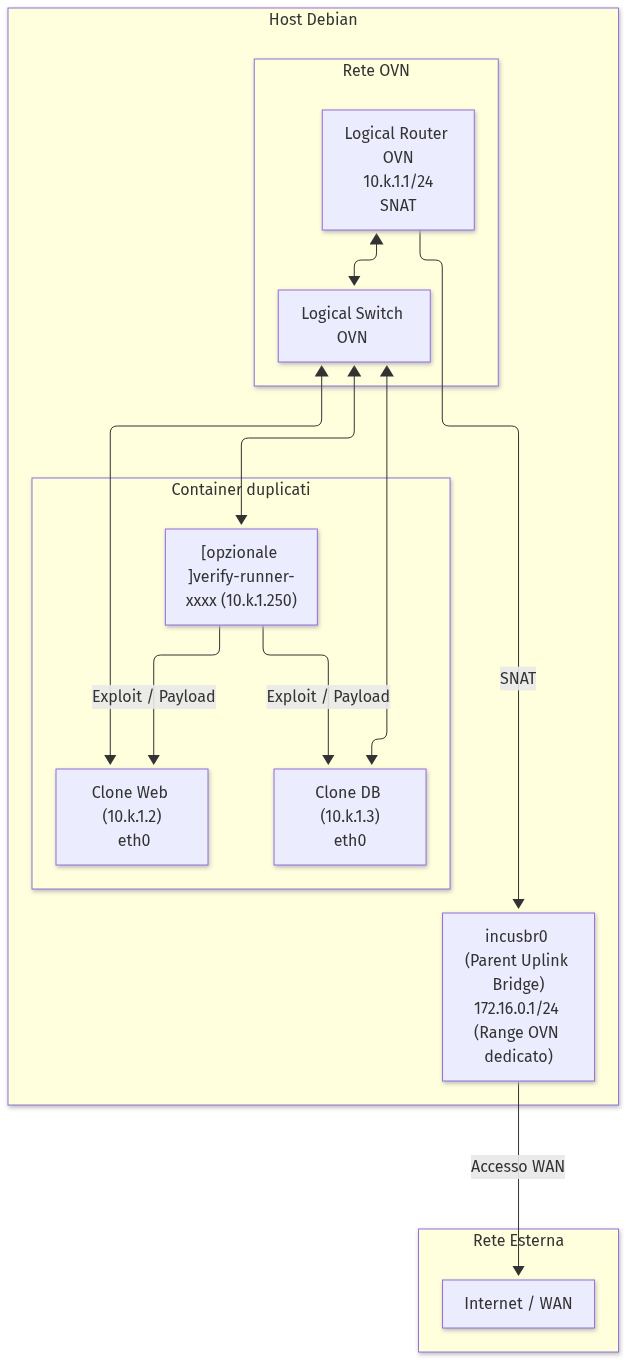
\includegraphics[width=0.92\linewidth,height=0.7\textheight,keepaspectratio]{src/images/mermaid_262_rete_verify_k_d80ab1c21b.png}
  \caption{262 Rete Verify K}
  \label{fig:mermaid_262_rete_verify_k_d80ab1c21b}
\end{figure}


\subsection{Architettura del codice}\label{architettura-del-codice}

A livello software, BlueAgent organizza l\textquotesingle interazione
con l\textquotesingle host disaccoppiando l\textquotesingle API in
\passthrough{\lstinline!/api!} dalla gestione a basso livello dei
container e delle componenti di rete, gestita ad alto livello dai
servizi in \passthrough{\lstinline!/services!}, che contiene la logica
di business, mentre le complessità operative sono delegate a moduli e
driver specializzati (\textbf{aggiungi cartelle}).

\begin{center}\rule{0.5\linewidth}{0.5pt}\end{center}

\subsubsection{\texorpdfstring{Astrazione del Runtime:
\texttt{ContainerEngine}}{Astrazione del Runtime: ContainerEngine}}\label{astrazione-del-runtime-containerengine}

BlueAgent non invoca direttamente il demone Incus
all\textquotesingle interno della logica delle challenge. Tutte le
operazioni di gestione del ciclo di vita dei container sono intermediate
da un\textquotesingle interfaccia astratta denominata
\passthrough{\lstinline!ContainerEngine!}.

Questa classe astratta formalizza esclusivamente le primitive necessarie
ai requisiti operativi del Cyber Range:

\begin{itemize}
\tightlist
\item
  Creazione, avvio, arresto forzato ed eliminazione delle istanze.
\item
  Duplicazione rapida e gestione delle interfacce di rete.
\item
  Esecuzione dei comandi nei container.
\end{itemize}

Disaccoppiare l\textquotesingle interfaccia
dall\textquotesingle implementazione permette ai servizi di non dover
conoscere come avviene la gestione dei container, e di predisporre il
codice per poter utilizzare altri gestori.

\begin{quote}
\textbf{ATTENZIONE: anche la generazione delle immagini dovrebbe
avvenire tramite interfaccia}
\end{quote}

L\textquotesingle implementazione concreta
\passthrough{\lstinline!IncusEngine!} comunica con il demone di sistema
tramite Unix Domain Socket
(\passthrough{\lstinline!/var/lib/incus/unix.socket!}), traducendo le
primitive astratte in chiamate REST HTTP asincrone.

\begin{quote}
\passthrough{\lstinline!Unix Domain Socket (UDS)!}: Meccanismo di
Inter-Process Communication (IPC) gestito interamente dal kernel del
sistema operativo. La comunicazione avviene trasferendo i dati
direttamente tra i buffer di memoria dei processi nello spazio kernel
senza attraversare lo stack di rete. L\textquotesingle endpoint è
rappresentato da un file speciale sul filesystem (es:
\passthrough{\lstinline!/var/lib/incus/unix.socket!}).\footnote{\label{fn:ref_21}Linux
  manual page, unix(7) - Sockets for local interprocess communication:
  \url{https://man7.org/linux/man-pages/man7/unix.7.html}}
\end{quote}

\begin{center}\rule{0.5\linewidth}{0.5pt}\end{center}

\subsubsection{\texorpdfstring{Ciclo di Vita della Sandbox: Async
Context Manager
(\texttt{OVNVerifier})}{Ciclo di Vita della Sandbox: Async Context Manager (OVNVerifier)}}\label{ciclo-di-vita-della-sandbox-async-context-manager-ovnverifier}

Il processo di verifica richiede di istanziare una replica fedele della
rete di produzione che deve esistere esclusivamente per la durata dei
test. In caso di qualsiasi tipo di fallimento,
l\textquotesingle infrastruttura clonata deve essere rilasciata per
evitare risorse allocate e sprecate.

Per garantire questa proprietà, il ciclo di vita della sandbox è
incapsulato all\textquotesingle interno della classe
\passthrough{\lstinline!OVNVerifier!}, implementata come
\textbf{Asynchronous Context Manager} di Python.

\begin{quote}
\textbf{Pattern RAII (Resource Acquisition Is Initialization):}
L\textquotesingle allocazione delle risorse è vincolato
dall\textquotesingle acquisizione del contesto, mentre il loro rilascio
e smantellamento deterministico è garantito all\textquotesingle uscita
dal blocco, gestendo automaticamente qualsiasi anomalia o interruzione.
{[}\^{}8{]}
\end{quote}

Il ciclo di vita dell\textquotesingle{}
\passthrough{\lstinline!OVNVerifier!} segue tre fasi:

\begin{enumerate}
\def\labelenumi{\arabic{enumi}.}
\tightlist
\item
  \textbf{Inizializzazione (\passthrough{\lstinline!\_\_aenter\_\_!}):}

  \begin{itemize}
  \tightlist
  \item
    Creazione della rete OVN temporanea
  \item
    Duplicazione dei container tramite snapshot ZFS
  \item
    Riconnessione dell\textquotesingle interfaccia
    \passthrough{\lstinline!eth0!} dei cloni alla nuova rete OVN
  \item
    Istanziazione opzionale del container \emph{Verifier Runner}.
  \end{itemize}
\item
  \textbf{Esecuzione delle Verifiche
  (\passthrough{\lstinline!run\_checks!}):}

  \begin{itemize}
  \tightlist
  \item
    Esecuzione controllata dei comandi di test con timeout
  \end{itemize}
\item
  \textbf{Rilascio e Teardown
  (\passthrough{\lstinline!\_\_aexit\_\_!}):}

  \begin{itemize}
  \tightlist
  \item
    Smantellamento delle risorse:

    \begin{enumerate}
    \def\labelenumii{\arabic{enumii}.}
    \tightlist
    \item
      Arresto ed eliminazione del container
      \passthrough{\lstinline!verify-runner!};
    \item
      Arresto forzato ed eliminazione di tutti i container cloni;
    \item
      Eliminazione della rete virtuale OVN.
    \end{enumerate}
  \end{itemize}
\end{enumerate}

L\textquotesingle uso dell\textquotesingle{}\textbf{Async Context
Manager} fornisce dunque un metodo sicuro per utilizzare
l\textquotesingle oggetto \passthrough{\lstinline!OVNVerifier!}

\begin{center}\rule{0.5\linewidth}{0.5pt}\end{center}

\subsubsection{Concorrenza e Two-Tier
Locking}\label{concorrenza-e-two-tier-locking}

Incus non supporta operazioni di mutazione concorrenti sul medesimo
container: qualora giungano due richieste simultanee, il demone Incus
rifiuta la transazione. Inoltre potrebbero nascere altri problemi
nell\textquotesingle accesso alle risorse dei team

Per prevenire questo fenomeno, BlueAgent implementa un meccanismo di
sincronizzazione a due livelli (\passthrough{\lstinline!TwoTierLock!}):

\begin{itemize}
\tightlist
\item
  \textbf{Tier 1 (Intra-processo):} utilizza
  \passthrough{\lstinline!asyncio.Lock!} per coordinare e serializzare
  le coroutine concorrenti all\textquotesingle interno del singolo event
  loop.
\item
  \textbf{Tier 2 (Inter-processo):} applica un lock non bloccante sul
  filesystem (\passthrough{\lstinline!fcntl.flock!}) memorizzato nel
  file \passthrough{\lstinline!/tmp/blueagent\_locks/<risorsa>.lock!}.
\end{itemize}

Questa architettura protegge le risorse sia a livello di singolo
processo sia in presenza di server ASGI multi-worker (come Uvicorn o
Gunicorn configurati con molteplici worker di sistema), garantendo mutua
esclusione sulle mutazioni dei container senza bloccare
l\textquotesingle event loop asincrono.

\begin{center}\rule{0.5\linewidth}{0.5pt}\end{center}

\subsubsection{Pipeline Asincrona non Bloccante su Socket
Unix}\label{pipeline-asincrona-non-bloccante-su-socket-unix}

Le operazioni di virtualizzazione (clonazione di storage, avvio di init
system complessi nei container di sistema, polling delle operazioni)
comportano latenze nell\textquotesingle ordine di decine o centinaia di
millisecondi. L\textquotesingle adozione di un modello sincrono
multithread comporterebbe un consumo eccessivo di risorse e colli di
bottiglia sotto carico.

BlueAgent è progettato secondo un paradigma completamente asincrono:

\begin{itemize}
\tightlist
\item
  \passthrough{\lstinline!IncusEngine!} comunica con il socket UDS
  locale (\passthrough{\lstinline!/var/lib/incus/unix.socket!}) per
  mezzo di \passthrough{\lstinline!httpx.AsyncClient!}.
\item
  Poiché le operazioni di mutazione in Incus sono gestite in background
  dal demone e restituiscono un UUID di tracciamento, BlueAgent
  interroga asincronamente l\textquotesingle endpoint
  \passthrough{\lstinline!/1.0/operations/<uuid>/wait!}, evitando cicli
  di polling bloccanti.
\item
  Le chiamate verso il kernel Linux (\passthrough{\lstinline!nftables!},
  \passthrough{\lstinline!ip link!}, WireGuard) sfruttano
  \passthrough{\lstinline!asyncio.create\_subprocess\_exec!}.
\end{itemize}

Questo approccio consente a un singolo processo BlueAgent di servire le
richieste di telemetria e validazione di centinaia di utenti con un
overhead di memoria e CPU quasi nullo.

\begin{center}\rule{0.5\linewidth}{0.5pt}\end{center}

\subsubsection{\texorpdfstring{Resilienza e Riconciliazione dello Stato
(\texttt{LifecycleManager})}{Resilienza e Riconciliazione dello Stato (LifecycleManager)}}\label{resilienza-e-riconciliazione-dello-stato-lifecyclemanager}

Qualora l\textquotesingle host subisca un riavvio forzato improvviso o
il processo di BlueAgent venga terminato bruscamente con
\passthrough{\lstinline!SIGKILL!}, le routine di pulizia
(\passthrough{\lstinline!\_\_aexit\_\_!}) non possono intervenire,
lasciando container e switch virtuali orfani sul sistema.

Per risolvere queste anomalie senza intervento manuale, BlueAgent
include il demone in background
\passthrough{\lstinline!LifecycleManager!}:

\begin{itemize}
\tightlist
\item
  Scansiona periodicamente le istanze e le reti con prefisso
  \passthrough{\lstinline!verify-*!} presenti su Incus, confrontandole
  con lo stato persistito nel database e forzandone
  l\textquotesingle eliminazione se non risultano associate a sessioni
  attive.
\item
  \textbf{Grace Period di 90 Secondi:} il demone ignora qualsiasi
  risorsa la cui creazione risalga a meno di 90 secondi. Questa finestra
  temporale risolve una race condition fondamentale: durante
  l\textquotesingle avvio di una verifica, la rete OVN viene creata
  prima che i container cloni vi siano collegati. Senza il periodo di
  grazia, il ciclo di bonifica interpreterebbe la rete appena creata
  come una risorsa "vuota e orfana", distruggendola mentre la richiesta
  legittima ne sta ancora completando la configurazione.
\end{itemize}

\begin{center}\rule{0.5\linewidth}{0.5pt}\end{center}
